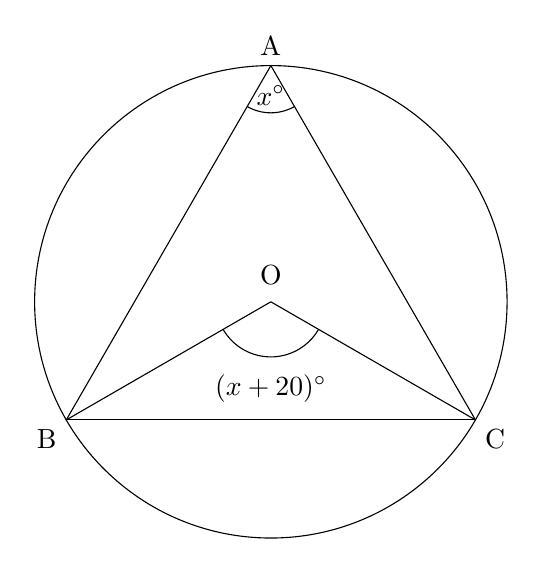
\begin{tikzpicture}

    % Define the radius of the circle
    \def\radius{3}
    
    % Define the center of the circle
    \coordinate (O) at (0, 0);
    
    % Define points A, B, C on the circle
    % A is at the top (90 degrees)
    \coordinate (A) at (90:\radius);
    
    % B is at the bottom left (210 degrees)
    \coordinate (B) at (210:\radius);
    
    % C is at the bottom right (330 degrees)
    \coordinate (C) at (330:\radius);

    % Draw the circle
    \draw (O) circle (\radius);

    % Draw the triangle ABC (inscribed in the circle)
    \draw (A) -- (B);
    \draw (B) -- (C);
    \draw (C) -- (A);

    % Draw lines from center O to vertices B and C
    \draw (O) -- (B);
    \draw (O) -- (C);

    % Draw arc for angle x at vertex A (angle BAC)
    % Angle from A to B is 210-90+180 = 240 degrees from A's perspective
    % Angle from A to C is 330-90+180 = 300 degrees from A's perspective
    \draw (A) ++(-60:0.6) arc (-60:-120:0.6);

    % Draw arc for angle (x+20) at center O (angle BOC)
    % Angle from O to C is 330 degrees, from O to B is 210 degrees
    \draw (O) ++(330:0.7) arc (330:210:0.7);

    % Label point A at the top
    \node[above] at (A) {A};
    
    % Label point B at the bottom left
    \node[below left] at (B) {B};
    
    % Label point C at the bottom right
    \node[below right] at (C) {C};
    
    % Label center O
    \node[above] at (0, 0.1) {O};

    % Label the angle x at vertex A
    \node at (0, 2.62) {$x^{\circ}$};

    % Label the angle (x+20) at center O
    \node at (0, -1.1) {$(x + 20)^{\circ}$};

\end{tikzpicture}